\documentclass[conference]{IEEEtran}
% Upload pipeline.png, accuracy.png and loss.png into a folder named "figures" in the Overleaf project
% (or upload paper/CSE-Tutor_overleaf.zip, which contains everything).
\usepackage[T1]{fontenc}
\usepackage{amsmath,amssymb}
\usepackage{graphicx}
\usepackage{booktabs}
\usepackage{array}
\usepackage{cite}
\usepackage{url}
\usepackage[hidelinks]{hyperref}

\newcommand{\ra}{$\rightarrow$}

\begin{document}

\title{CSE-Tutor: Verified Synthetic Data and Explanation-Style Training for a 1.5B-Parameter Computer Science Tutor}

\author{\IEEEauthorblockN{Satya Dedeepya}
\IEEEauthorblockA{Course project, Deep Learning\\
\url{github.com/satyadedeepya/slm_dl_project}}}

\maketitle

\begin{abstract}
Small language models can run privately on a student's laptop, but they are unreliable on the numerical problems that dominate computer-science examinations and their explanations are uneven. We fine-tune Qwen2.5-1.5B-Instruct with LoRA as a tutor for six subjects (data structures and algorithms, programming, databases, operating systems, computer networks and deep learning). The distinctive part of the training data is \emph{programmatically verified}: 3,000 problems from 41 generators whose step-by-step solutions are computed by running the underlying algorithm and are cross-checked against textbook examples and PyTorch. All training and evaluation run on an integrated Intel Arc GPU. On held-out tests the first fine-tuned model significantly improves text-to-SQL execution accuracy (50.5\ra 60.0), functional-dependency problems (15\ra 30) and network numericals (1\ra 8) over the base model (exact McNemar $p<0.05$) without loss on code generation, and an ablation that removes only the verified data removes these gains. A continued-training stage adds deep learning without forgetting. Because accuracy does not measure explanation quality, we add a blind, order-balanced pairwise judge on 39 held-out questions. It shows that fine-tuning on short targets made concept explanations worse than the base model's (6--13); two explanation-style stages trained on teaching-format answers raise answer length from 79 to 194 words and narrow, but do not close, this gap (6--11--3, not significant), while the final model is significantly more accurate than the base model on four of five tasks (DBMS 15\ra 35, DL 2\ra 13, CN 1\ra 11, Spider 50.5\ra 59.0) and wins numerical solutions 13--5.
\end{abstract}

\begin{IEEEkeywords}
small language models, LoRA, synthetic data, data verification, LLM-as-a-judge, computer science education, text-to-SQL
\end{IEEEkeywords}

\section{Introduction}
Students preparing for university examinations, GATE and placement interviews need an assistant that explains concepts, solves numerical problems step by step and writes correct code and SQL. Large hosted models do this well but cost money, need connectivity and send student data to a third party. A 1.5B-parameter model runs locally on an ordinary laptop, but out of the box it computes CPU-scheduling waiting times, page faults and subnet ranges incorrectly: it pattern-matches the shape of a solution instead of executing the procedure.

The common recipe for adapting a small model is to fine-tune it on question--answer pairs written by a larger model~\cite{selfinstruct,glan,orca}. Such labels are unverified, and a small student model can learn the teacher's mistakes. For the algorithmic part of the curriculum we take a different route: we write generators that sample random problem instances and \emph{compute} their solutions by running the algorithm, so every label is correct by construction. For the conceptual part we use teacher answers, but filter them against answer keys and, in later stages, rewrite them into a fixed teaching format.

We ask four research questions:
\begin{itemize}
\item \textbf{RQ1:} how much does LoRA fine-tuning improve a 1.5B model on CS tasks compared with zero- and few-shot prompting?
\item \textbf{RQ2:} does the verified numerical data cause the improvement on numerical problems, or does the rest of the mix?
\item \textbf{RQ3:} can a new subject (deep learning) be added cheaply by continued training without forgetting earlier skills?
\item \textbf{RQ4:} does the fine-tuned tutor \emph{explain} better than the base model, not only answer more accurately, and can explanation-style training fix it if it does not?
\end{itemize}
Our contributions are: (1) verified generators for 41 problem types across operating systems, networks, databases and deep learning, tested against textbook examples and PyTorch; (2) a controlled ablation isolating the effect of the verified data; (3) a statistically careful evaluation on seven held-out benchmarks (bootstrap confidence intervals, exact McNemar tests, format failures counted separately); (4) a blind, order-balanced pairwise evaluation of explanation quality, and two explanation-style training stages measured with it; (5) an error taxonomy of the fine-tuned model; and (6) a local chat interface that serves all model variants. Everything, including five training runs, runs on a laptop with an integrated GPU.

The main findings are that verified data is what teaches procedures (RQ2), that a short continued-training stage with replay adds a subject without forgetting (RQ3), and that the \emph{length and format of the training targets} largely decide how the model explains (RQ4): training on short answers made the tutor more accurate but terser than the base model, and longer teaching-format targets recover most, but not all, of the base model's explanation quality.

\section{Related Work}
\emph{Parameter-efficient fine-tuning.} LoRA~\cite{lora} trains low-rank updates of frozen weights; QLoRA~\cite{qlora} additionally quantises the base model to 4 bits. We use LoRA on all attention and MLP projections of Qwen2.5-1.5B-Instruct~\cite{qwen25,qwencoder}. Continued training of one adapter across stages is closely related to rehearsal methods for continual learning~\cite{replay}: we mix replay data from earlier stages into each new stage.

\emph{Language models for CS education.} GuideLM~\cite{guidelm} shows that small supervised sets shape pedagogical behaviour; QLoRA has been applied to data-structures problems~\cite{dsaqlora}; local open-source teaching assistants are studied in~\cite{aita,smallmodels,vta}. CS-Bench~\cite{csbench} is the closest benchmark and serves as our multiple-choice evaluation.

\emph{Synthetic and distilled instruction data.} Self-Instruct~\cite{selfinstruct} and GLAN~\cite{glan} generate instruction data with language models, and Orca~\cite{orca} shows that training on a teacher's step-by-step explanation traces transfers reasoning style to smaller models. LIMA~\cite{lima} argues that alignment mostly teaches a model the \emph{format} of answers, which matches our observation that answer length and structure follow the training targets. Our generators are programs, so their correctness does not depend on a teacher; program-aided reasoning~\cite{pal} is the natural next step for the arithmetic errors that remain.

\emph{Evaluating explanations.} Strong language models can serve as judges of open-ended answers, but they show position and verbosity biases~\cite{mtbench}; we therefore judge every pair in both orders, hide model names, instruct the judge not to reward length and count a win only when both orders agree. Preference optimisation such as DPO~\cite{dpo} is a natural follow-up once such comparisons exist.

\emph{Forgetting.} Parameter-efficient tuning still forgets~\cite{forgetting}. We keep replay data in every stage and re-measure code generation and SQL after every stage.

\section{System Overview}
Fig.~\ref{fig:pipeline} shows the pipeline. Data come from four kinds of sources with different quality gates. Five LoRA runs are trained: FT-A and FT-B from the base model (the ablation pair), then FT-C, FT-D and FT-E as continued-training stages, each starting from the previous adapter. Every run is evaluated with the same harness, and all adapters are served side by side by one chat server.

\begin{figure*}[t]
\centering
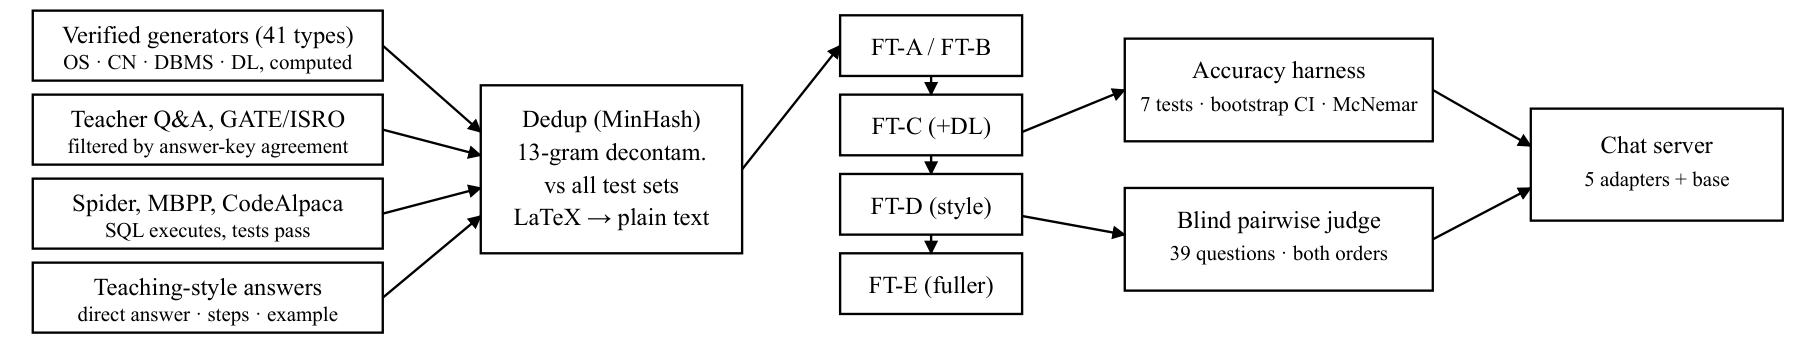
\includegraphics[width=0.95\textwidth]{figures/pipeline.png}
\caption{Pipeline: data sources and quality gates, the five LoRA runs (each continued stage starts from the previous adapter), the two evaluations and the chat server.}
\label{fig:pipeline}
\end{figure*}

\section{Data}
\subsection{Verified generators}
Each generator samples parameters, runs the algorithm and writes a solution in a fixed teaching format that ends with a \texttt{Final answer:} line, plus a machine-readable grading specification (Table~\ref{tab:gen}). Questions state their conventions (tie-breaking, whether C-SCAN counts the return seek, whether parameters include biases) so that the reference answer is unambiguous. Test problems are drawn from parameter pools disjoint from training and from a different random seed. Correctness is checked by unit tests against textbook worked examples (e.g.\ Silberschatz scheduling and page-replacement figures), by property tests (Belady's optimality, validity of safety sequences), and, for deep learning, by recomputing every answer type with PyTorch layers and autograd.

\begin{table}[t]
\centering
\caption{Verified generator families}
\label{tab:gen}
\begin{tabular}{@{}l p{4.3cm} r@{}}
\toprule
Subject & Families & Train / test \\
\midrule
OS & scheduling (6 algorithms), page replacement, Banker's, disk scheduling & 900 / 100 \\
CN & subnetting, CRC, checksum, delays, sliding window & 900 / 100 \\
DBMS & closure, candidate keys, normal form, lossless join & 600 / 100 \\
DL & conv/pool shapes, MLP parameters, forward pass, softmax-CE, GD, backprop, momentum, attention, P/R/F1 & 600 / 100 \\
\bottomrule
\end{tabular}
\end{table}

\noindent\fbox{\parbox{0.96\columnwidth}{\small\textsc{Example generated problem (DL, test split).} A convolutional layer receives an input of size $227\times227\times6$. It has 20 filters of size $11\times11$, stride 2 and padding 5. Find the output size and the number of trainable parameters (including biases).\\[2pt]
Reference (computed): $\lfloor(227+2\cdot5-11)/2\rfloor+1=114$, so $114\times114\times20$; parameters $(11\cdot11\cdot6+1)\cdot20=14{,}540$. Grading spec: numbers [114, 114, 20, 14540].}}

\subsection{First-stage training mix}
The first-stage mix (9,335 examples, 2.68M tokens; Table~\ref{tab:mix}) combines the generators with GATE/ISRO previous-year questions whose explanations were produced by a teacher model \emph{without the key} and kept only when the teacher agreed with the official answer (990 of 1,154), concept Q\&A over a 133-topic syllabus (multiple-choice and true/false items kept only on key agreement), Q\&A grounded in four openly licensed textbooks, Spider~\cite{spider} text-to-SQL with real schemas, MBPP~\cite{mbpp} and CodeAlpaca for code, and general replay data. All sources are deduplicated with MinHash and decontaminated against every evaluation set with 13-gram overlap. GATE papers up to 2020 and half of 2021--2026 are used for training; the other half of 2021--2026 is held out.

\begin{table}[t]
\centering
\caption{First-stage training mix (train + validation)}
\label{tab:mix}
\begin{tabular}{@{}l r l@{}}
\toprule
Source & Examples & Quality gate \\
\midrule
Verified generators (OS, CN, DBMS) & 2,400 & computed answers \\
GATE / ISRO PYQs & 978 & teacher agrees with key \\
Concept Q\&A (teacher) & 1,458 & MCQ/TF key agreement \\
Open-textbook Q\&A & 1,170 & answerable from passage \\
Spider & 1,335 & gold SQL executes \\
MBPP / CodeAlpaca & 311 / 1,184 & tests pass / code parses \\
Replay (Alpaca) & 499 & length filter \\
\bottomrule
\end{tabular}
\end{table}

\subsection{Deep-learning stage}
The DL stage (2,107 examples, 0.61M tokens) contains 600 verified DL problems, 307 DL concept Q\&A items over 36 syllabus topics (teacher-generated, filtered by key agreement) and 1,200 replay examples sampled from the first-stage mix, so that the earlier skills are rehearsed while the new subject is learned.

\subsection{Explanation-style stages}
An inspection of the training targets explained why the tutor's concept answers were terse: teacher concept answers had a median of 57--91 words and code/SQL targets 15--25 words, against about 290 words in the base model's own answers, and 291 targets contained \LaTeX. We therefore built a teaching-style set of about 1,340 questions (every open concept question plus ``What is \emph{X}?'' and ``Explain \emph{X} with an example'' for all 169 syllabus topics). A teacher model answers each one in a fixed format: a direct answer in one or two sentences, numbered key points with short bold labels, one worked example (numbers, a small table, a code snippet or a trace) and a closing ``In short:'' line; mathematics is written as plain Unicode text, never \LaTeX. Questions whose word overlap with any evaluation question has Jaccard similarity of at least 0.4 are removed (12 questions). The FT-D set uses these answers as written (median 164 words). For FT-E, every answer under 220 words was rewritten into a 250--350-word version that explains each point and adds a worked example and a common mistake, giving a median of 286 words. All targets are converted to plain-text mathematics; none contains \LaTeX.

\section{Training}
\emph{Setup.} LoRA rank 16, $\alpha=32$, dropout 0.05 on the q, k, v, o, gate, up and down projections (18.5M trainable parameters, 1.18\%); loss on assistant tokens only; AdamW with cosine decay and 3\% warm-up; effective batch 32 (batch 1 $\times$ 32 accumulation); one epoch per stage; bf16; length-grouped batches; maximum length 1,024 tokens. Continued stages load the previous adapter as trainable and use a lower learning rate (Table~\ref{tab:runs}).

\emph{Hardware.} An Intel Core Ultra 5 125H with integrated Arc graphics and 8.4\,GB of shared memory. bitsandbytes 4-bit quantisation is not dependable on Intel XPU, so the base model is held in bf16 (the adapter is the same as in QLoRA). Batch 4 ran out of memory because the 152K-token vocabulary makes the logits alone about 2.5\,GB, hence gradient accumulation. Long runs were made robust to sleep and power events with checkpoint-and-resume and a keep-awake wrapper.

\begin{table*}[t]
\centering
\caption{Training runs. Each continued stage starts from the adapter in the ``Init'' column. Validation sets differ per stage, so losses are not comparable across rows.}
\label{tab:runs}
\begin{tabular}{@{}l l l r r l r r@{}}
\toprule
Run & Init & Training data & Examples & Steps & LR & Time & Val.\ loss \\
\midrule
FT-A & base & first-stage mix without generator data (ablation) & 6,588 & 206 & $2\times10^{-4}$ & 3.7 h & 0.95 \\
FT-B & base & full first-stage mix & 8,868 & 278 & $2\times10^{-4}$ & 4.8 h & 0.65 \\
FT-C & FT-B & DL problems + DL concepts + 1,200 replay & 2,107 & 66 & $10^{-4}$ & 70 min & 0.46 \\
FT-D & FT-C & 1,192 teaching-style answers + 1,050 verified + 250 code/SQL replay & 2,492 & 78 & $10^{-4}$ & 96 min & 0.79 \\
FT-E & FT-D & 1,254 fuller teaching-style answers + 450 verified + 100 code/SQL replay & 1,804 & 57 & $10^{-4}$ & 81 min & 0.68 \\
\bottomrule
\end{tabular}
\end{table*}

\section{Evaluation Protocol}
\emph{Accuracy.} Adapters are merged and decoded greedily with the same prompts for every model (Table~\ref{tab:evalsets}). B0 and B1 are the base model prompted zero-shot and 3-shot. We report 95\% bootstrap confidence intervals~\cite{efron} and exact two-sided McNemar tests~\cite{mcnemar} on paired items, and count unparseable answers separately so that learning the answer format is not mistaken for knowledge. For DL numericals we also report value-level accuracy, the share of expected numbers that appear in the final answer, with a paired sign-flip permutation test.

\begin{table}[t]
\centering
\caption{Held-out evaluation sets}
\label{tab:evalsets}
\begin{tabular}{@{}l r l@{}}
\toprule
Test & $n$ & Metric \\
\midrule
CS-Bench DSA/OS/CN~\cite{csbench} & 400 & MCQ and T/F accuracy \\
Verified OS / CN / DBMS / DL & 100 each & exact match (typed grader) \\
MBPP test~\cite{mbpp} & 200 & pass@1 with tests \\
Spider dev~\cite{spider} & 200 & execution accuracy \\
GATE CS 2021--26 (held-out half) & 56 & MCQ accuracy \\
Explanation set (RQ4) & 39 & blind pairwise judgement \\
\bottomrule
\end{tabular}
\end{table}

\emph{Explanation quality.} Final-answer accuracy does not measure whether an answer teaches. The explanation set has 39 held-out questions: 19 verified numericals (one per problem type; DBMS has four types) with their reference solutions, and 20 concept questions of the kind students type into the chat interface (``What is CNN?'', ``Explain the TCP three-way handshake''). Each model answers with the training system prompt and greedy decoding, and answers are shown to the judge exactly as the chat interface shows them (\LaTeX{} converted to plain text). A fixed judge model (Gemma~4 31B) sees the question, the reference solution for numericals, and two answers labelled only A and B. It scores correctness, steps and clarity from 1 to 5 and names the better answer, with correctness weighted most and an explicit instruction not to prefer longer answers. Every pair is judged twice with the order swapped; a model wins a question only if it wins in both orders, and any disagreement counts as a tie. Significance of win--loss counts uses an exact sign test.

\section{Results}
\begin{table*}[t]
\centering
\caption{Accuracy (\%) on held-out tasks; --: not evaluated}
\label{tab:results}
\begin{tabular}{@{}l r r r r r r r r@{}}
\toprule
Task & $n$ & B0 0-shot & B1 3-shot & FT-A & FT-B & FT-C & FT-D & FT-E \\
\midrule
CS-Bench (DSA/OS/CN) & 400 & 51.2 & \textbf{58.0} & 53.8 & 55.2 & -- & -- & -- \\
OS numericals & 100 & 4.0 & 4.0 & 3.0 & 5.0 & -- & -- & -- \\
CN numericals & 100 & 1.0 & 2.0 & 0.0 & 8.0 & 7.0 & \textbf{12.0} & 11.0 \\
DBMS FD problems & 100 & 15.0 & 12.0 & 17.0 & 30.0 & 31.0 & 24.0 & \textbf{35.0} \\
DL numericals & 100 & 2.0 & -- & -- & 3.0 & 5.0 & \textbf{21.0} & 13.0 \\
MBPP pass@1 & 200 & 41.5 & 41.5 & 41.0 & \textbf{42.5} & 40.0 & 39.5 & 40.0 \\
Spider (execution) & 200 & 50.5 & -- & 54.5 & \textbf{60.0} & 59.5 & 58.5 & 59.0 \\
GATE CS 2021--26 & 56 & 33.9 & -- & \textbf{37.5} & 33.9 & -- & -- & -- \\
\bottomrule
\end{tabular}
\end{table*}

\begin{table*}[t]
\centering
\caption{Exact McNemar $p$-values against the zero-shot base model B0 (bold: $p<0.05$)}
\label{tab:pvals}
\begin{tabular}{@{}l r r r r r r@{}}
\toprule
Task & FT-A & FT-B & FT-C & FT-D & FT-E & FT-B vs FT-A \\
\midrule
CS-Bench & 0.42 & 0.18 & -- & -- & -- & 0.57 \\
CN numericals & 1.00 & \textbf{0.039} & 0.070 & \textbf{0.003} & \textbf{0.006} & \textbf{0.008} \\
DBMS FD problems & -- & \textbf{0.017} & \textbf{0.003} & 0.108 & \textbf{0.001} & 0.060 \\
DL numericals & -- & -- & 0.45 & \textbf{$<$0.001} & \textbf{0.007} & -- \\
MBPP & -- & 0.89 & 0.79 & 0.69 & 0.79 & 0.66 \\
Spider & -- & \textbf{0.011} & \textbf{0.015} & \textbf{0.029} & \textbf{0.019} & 0.052 \\
GATE & -- & 1.00 & -- & -- & -- & 0.82 \\
\bottomrule
\end{tabular}
\end{table*}

\begin{figure*}[t]
\centering
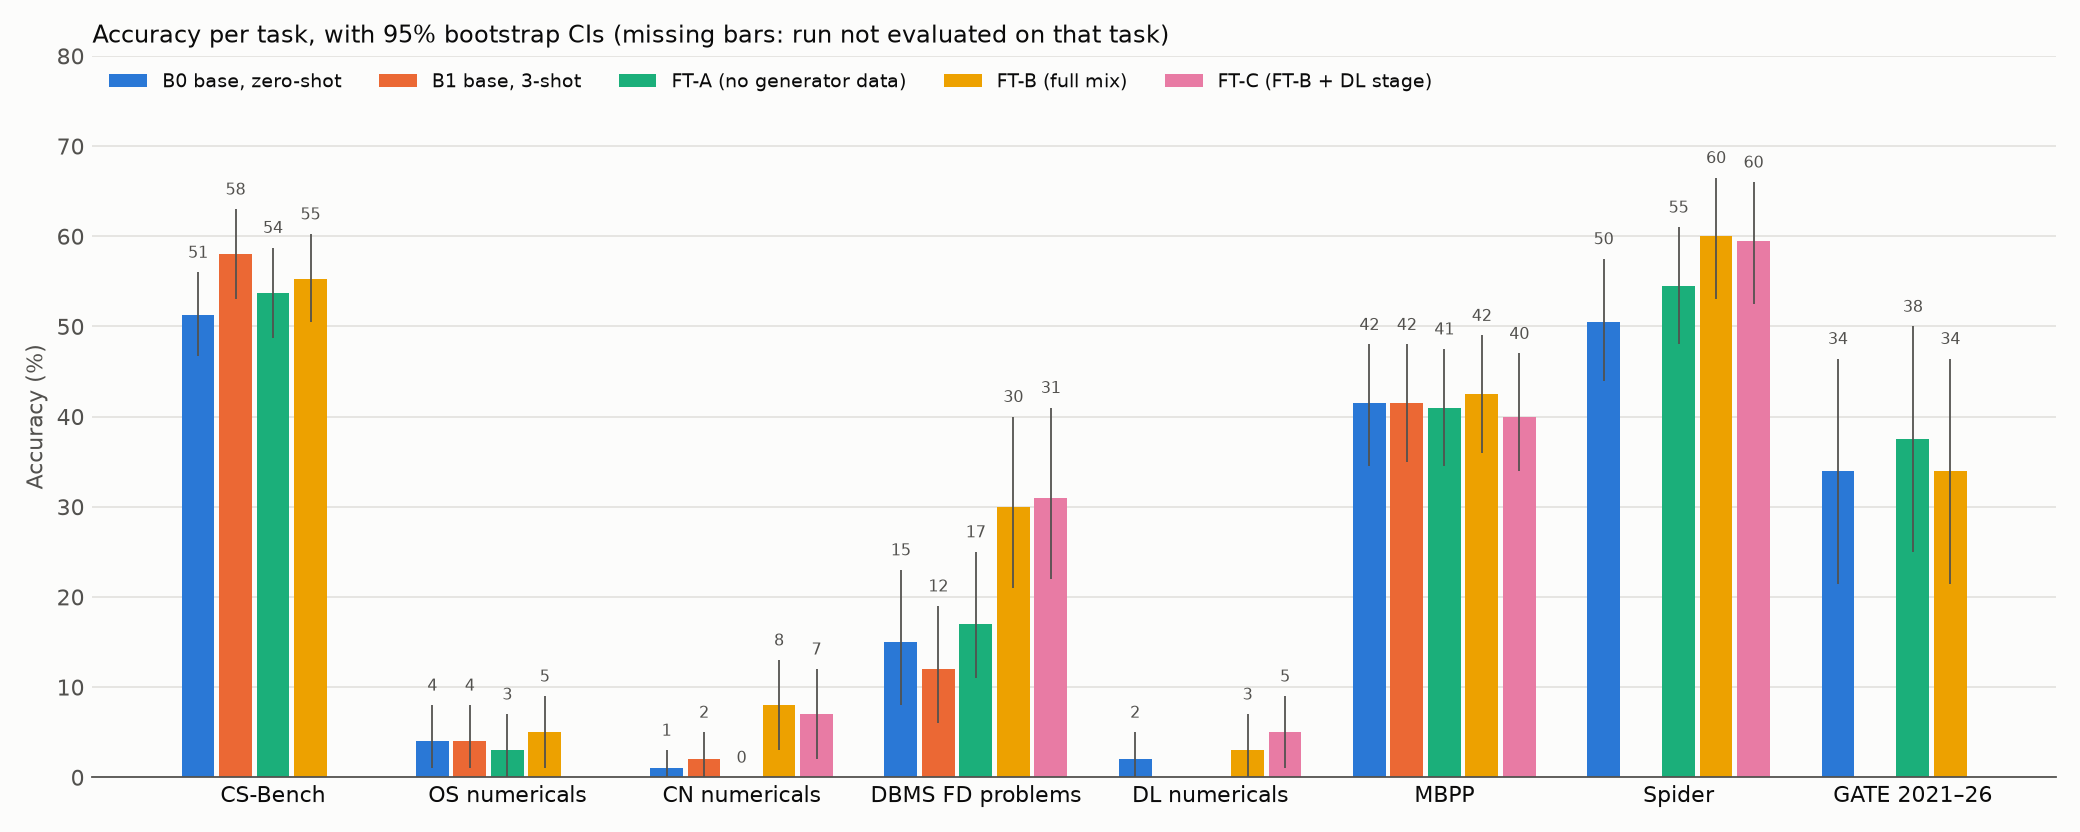
\includegraphics[width=0.9\textwidth]{figures/accuracy.png}
\caption{Accuracy per task with 95\% bootstrap confidence intervals. Missing bars: run not evaluated on that task (later stages were evaluated on the five most informative tasks).}
\label{fig:acc}
\end{figure*}

\subsection{RQ1: fine-tuning versus prompting}
FT-B significantly improves over the zero-shot base model on Spider (+9.5 points, $p=0.011$), DBMS functional-dependency problems (+15.0, $p=0.017$) and network numericals (+7.0, $p=0.039$) (Tables~\ref{tab:results} and~\ref{tab:pvals}, Fig.~\ref{fig:acc}). On CS-Bench the gain (+4.0) is not significant, and about half of it comes from fewer unparseable answers (21\ra 7 of 400); three-shot prompting remains slightly better on this knowledge-oriented benchmark. MBPP and GATE do not change significantly, so fine-tuning does not degrade code generation or examination performance. The only negative signal is CS-Bench's \emph{reasoning} subset, which fell by 6--7 points in both first-stage runs (not significant at $n=142$). OS numericals stay near the floor for every model.

\subsection{RQ2: what the verified data contributes}
FT-A, trained on the same mix and settings minus the generator slice, stays at base-model level on every numerical task (CN 0\%; closure and candidate keys 0\% versus 32.8\% for FT-B), and FT-B beats FT-A on CN numericals ($p=0.008$). The numerical gains are therefore caused by the verified data rather than by teacher Q\&A, textbooks or examination questions. On CS-Bench, MBPP and GATE the two runs are within noise: the generated data is specific in its effect. FT-B also trains for 35\% more steps than FT-A, so part of any FT-B--FT-A difference could come from training length; a step-matched control is left to future work. CPU and disk scheduling stay at 0\% for every model: FT-B reproduces Gantt charts and tables perfectly but fills them with wrong values.

\subsection{RQ3: adding deep learning by continued training}
The DL stage took 70\,min of training. Exact match on the 100 held-out DL problems is a harsh metric, because every number of a multi-part answer must be right; measured per expected value, FT-C produces 26.0\% of the correct values against 15.8\% for FT-B and 12.6\% for the base model (Table~\ref{tab:dl}), significant under a paired sign-flip permutation test ($p=0.013$ vs FT-B, $p=0.001$ vs B0). Value-level accuracy rises most for convolution shapes (22\ra 47\%), softmax/cross-entropy (0\ra 56\%) and classification metrics (22\ra 44\%), while one-step gradient descent (36\ra 8\%) and momentum (31\ra 19\%) get worse and attention and sigmoid back-propagation stay at 0\%. The stage did not erode earlier skills: against FT-B, DBMS, CN, Spider and MBPP differ by at most a few items (McNemar $p\ge0.38$). The later stages, which replay 450--1,050 verified problems, raised exact match on DL to 21\% (FT-D) and 13\% (FT-E).

\begin{table}[t]
\centering
\caption{DL numericals ($n=100$): exact and value-level accuracy (\%)}
\label{tab:dl}
\begin{tabular}{@{}l r l r@{}}
\toprule
Model & Exact & Values [95\% CI] & $p$ vs prev. \\
\midrule
B0 base & 2.0 & 12.6 [8.3--17.2] & -- \\
FT-B & 3.0 & 15.8 [11.0--20.8] & 0.27 \\
FT-C & 5.0 & \textbf{26.0} [19.8--32.2] & \textbf{0.013} \\
\bottomrule
\end{tabular}
\end{table}

\subsection{RQ4: explanation quality}
The blind comparison confirms what users of the chat interface noticed (Table~\ref{tab:pair}). FT-C wins the numericals 14--4 (sign test $p=0.031$) but loses the concept questions 6--13: it answers in a median of 79 words where the base model uses 286, and the judge rates its concept steps 2.65 and clarity 3.40 against 4.15 and 4.33 for the base model (Table~\ref{tab:scores}). Fine-tuning on short targets made the tutor more accurate but terser.

\begin{table}[t]
\centering
\caption{Blind pairwise comparison against the base model (win--loss--tie, sign-test $p$)}
\label{tab:pair}
\begin{tabular}{@{}l c c r@{}}
\toprule
Model & Numericals (19) & Concepts (20) & Words \\
\midrule
B0 base & -- & -- & 286 \\
FT-C & \textbf{14--4--1} (0.031) & 6--13--1 (0.17) & 79 \\
FT-D & \textbf{13--4--2} (0.049) & 8--12--0 (0.50) & 102 \\
FT-E & 13--5--1 (0.096) & 6--11--3 (0.33) & 194 \\
\bottomrule
\end{tabular}
\end{table}

\begin{table}[t]
\centering
\caption{Judge scores (1--5), model / base, averaged over both orders}
\label{tab:scores}
\begin{tabular}{@{}l l c c c@{}}
\toprule
Model & Set & Correct & Steps & Clarity \\
\midrule
FT-C & numer. & 1.79 / 1.53 & 2.68 / 1.92 & 3.47 / 2.71 \\
 & concept & 3.48 / 3.35 & 2.65 / 4.15 & 3.40 / 4.33 \\
\midrule
FT-D & numer. & 1.76 / 1.58 & 2.79 / 1.97 & 3.61 / 2.74 \\
 & concept & 3.50 / 3.40 & 3.17 / 3.95 & 3.85 / 4.28 \\
\midrule
FT-E & numer. & 1.74 / 1.58 & 2.87 / 2.00 & 3.61 / 2.79 \\
 & concept & 3.12 / 3.27 & 3.55 / 4.00 & 3.77 / 4.17 \\
\bottomrule
\end{tabular}
\end{table}

FT-D, trained on teaching-style answers, keeps the numerical advantage (13--4, $p=0.049$) and narrows the concept gap (8--12; steps 3.17 vs 3.95). Its accuracy on DL numericals rises from 5\% to 21\% (McNemar $p<0.001$ against FT-C), with no significant change elsewhere (DBMS 31\ra 24, $p=0.31$). FT-E, trained on fuller answers, writes a median of 194 words and reaches the highest concept-step score of any fine-tuned model (3.55 vs 4.00 for the base model), but the base model still wins slightly more concept questions (6--11--3, $p=0.33$) and FT-E's concept correctness is slightly lower (3.12 vs 3.27). FT-E is the most accurate model on DBMS (35\%, $p=0.001$ vs B0; $p=0.035$ vs FT-D) and remains significantly ahead of the base model on DL, CN and Spider, with code generation unchanged; compared with FT-D it trades DL accuracy (21\ra 13, $p=0.008$) for DBMS (24\ra 35). On numerical solutions, all fine-tuned models score higher than the base model on steps and clarity even when both final answers are wrong, because they apply the right procedure (Section~\ref{sec:example}).

\subsection{A worked example}\label{sec:example}
For the convolution problem in Section~IV-A, both the base model and FT-E give a wrong final answer, yet the judge prefers FT-E in both orders. The base model uses $\lfloor(N-K)/S\rfloor+1$, ignoring the padding, and omits the input channels from the parameter count. FT-E writes the correct formulas, $\lfloor(N+2P-K)/S\rfloor+1$ and $(K\cdot K\cdot C+1)\cdot F$, substitutes the right values and then slips on one subtraction:

\noindent\fbox{\parbox{0.96\columnwidth}{\small\textsc{FT-E (excerpt).}\\
\texttt{Output size per spatial dimension: }$\lfloor(N+2P-K)/S\rfloor+1$\\
$=\lfloor(227+2\cdot5-11)/2\rfloor+1=\lfloor219/2\rfloor+1=110$.\\
\texttt{Each filter has K x K x C weights plus one bias:} $11\cdot11\cdot6+1=737$.\\
\texttt{Parameters =} $737\times20=14740$.\\[2pt]
($227+10-11=226$, giving 114 and 14,540.) The judge's reason: ``uses the correct formulas \ldots\ and fails only on basic arithmetic, whereas [the base answer] uses incorrect formulas by ignoring padding and input channels.''}}

\smallskip
This pattern, a correct procedure with an arithmetic slip, is the most common failure of the fine-tuned models and motivates tool use for arithmetic.

\subsection{Cost}
The five training runs took about 12.6 hours on the laptop in total (Table~\ref{tab:runs}). Generation for the five-task accuracy evaluation of one adapter takes about 35--40 minutes with batched decoding; the explanation comparison for one model takes about 10 minutes of generation plus the judge calls. Interactive answers in the chat interface stream in 20--80 seconds.

\begin{figure*}[t]
\centering
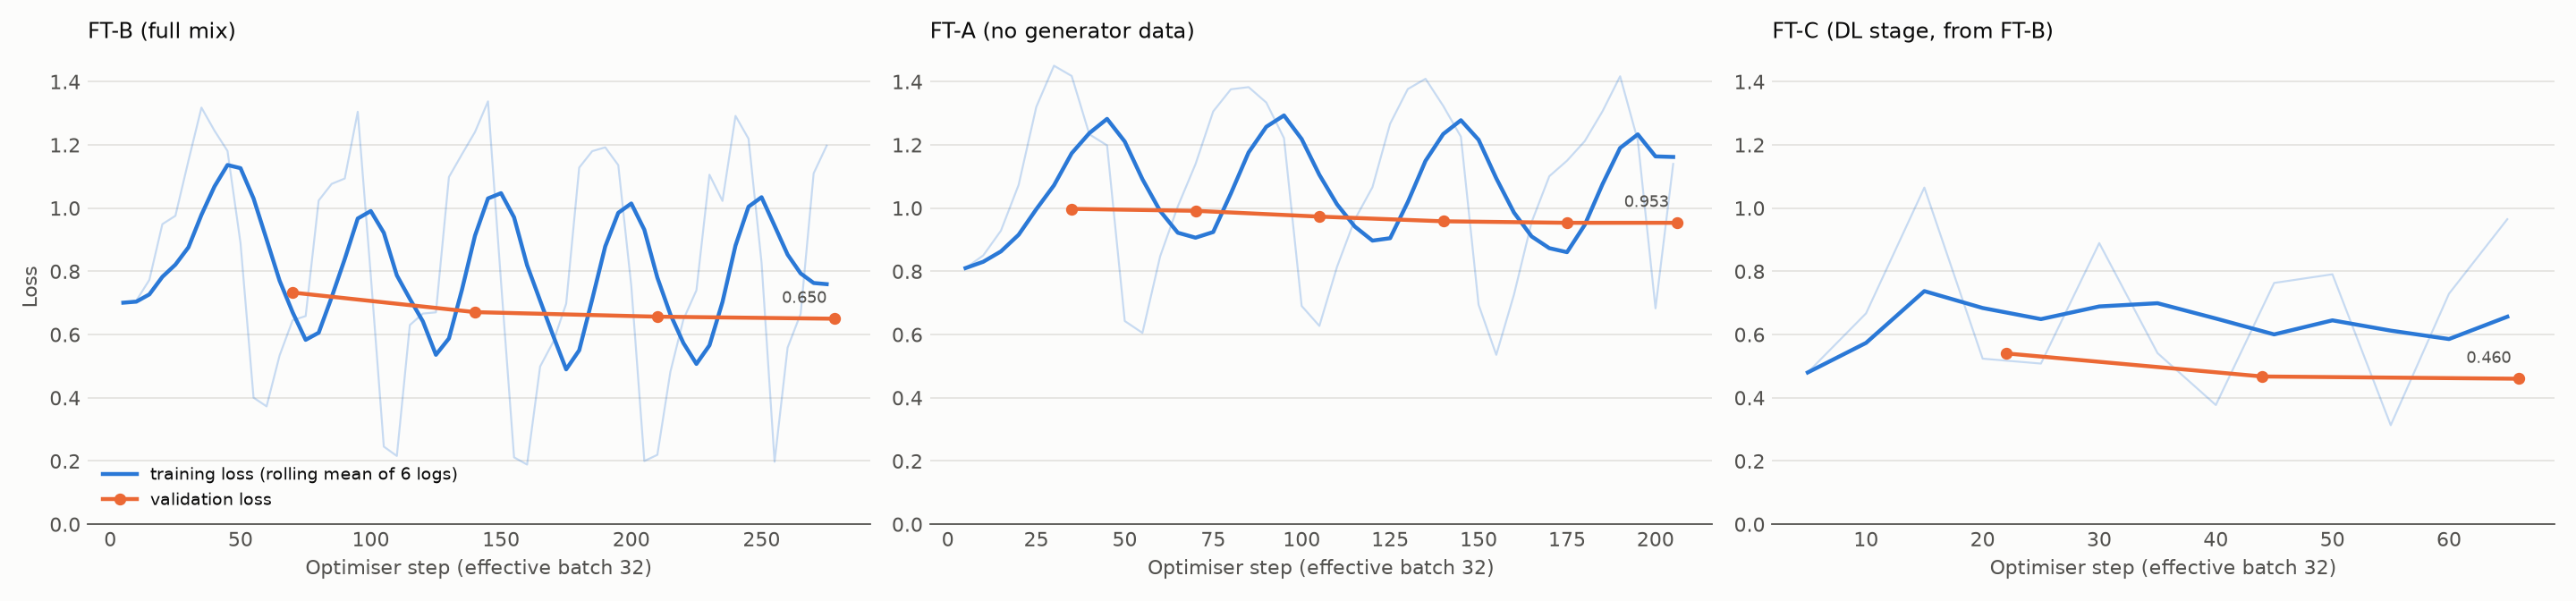
\includegraphics[width=0.9\textwidth]{figures/loss.png}
\caption{Training loss (rolling mean) and validation loss of the first-stage runs. The runs use different validation samples and are not directly comparable.}
\label{fig:loss}
\end{figure*}

\section{Error Analysis}\label{sec:errors}
We hand-labelled a stratified random sample of 50 wrong FT-B answers (12 CS-Bench, 8 each OS/CN/DBMS, 7 MBPP, 7 Spider) with one primary cause each (Table~\ref{tab:err}). None was a format failure.

\begin{table}[t]
\centering
\caption{Error categories of FT-B ($n=50$)}
\label{tab:err}
\begin{tabular}{@{}l r l@{}}
\toprule
Category & Share & Typical case \\
\midrule
Procedure / state tracking & 52\% & closure stops after one FD \\
Knowledge gap & 16\% & avoidance vs prevention \\
Schema hallucination & 12\% & column from wrong table \\
Arithmetic / units & 8\% & 0.96\,ms written as 9.6\,ms \\
Misread task & 6\% & number returned, bool expected \\
Answer contradicts reasoning & 4\% & argues A, answers B \\
Ambiguous item & 2\% & -- \\
\bottomrule
\end{tabular}
\end{table}

Procedure errors account for 20 of the 24 numerical failures and fall into three patterns: \emph{early stopping in fixed-point loops} (attribute closure applies one dependency and declares that nothing else applies), \emph{unfaithful reading of the input} (claiming an attribute never appears on a right-hand side when it does; ordering FCFS by process number instead of arrival) and \emph{inconsistent state} (LRU tables wider than the frame count; negative waiting times that are never checked). Spider failures are grounding errors against a schema that is in the prompt. In the explanation stages a second pattern appears in open answers: the structure is right but an invented example or a loosely worded point lowers correctness, for example a CNN ``example trace'' that does not compute a real convolution.

\section{Discussion}
\emph{Targets decide behaviour.} The clearest lesson is that the model reproduces the shape of its training targets. Short teacher answers produced a terse tutor (79 words); teaching-format answers of median 164 and 286 words produced answers of 102 and 194 words with the same structure. This is consistent with the view that fine-tuning mainly teaches format~\cite{lima}, and it means explanation quality has to be designed into the data, not hoped for.

\emph{Verified data teaches procedures, not arithmetic.} Verified generators are the only source that moved numerical accuracy, and every later stage that replayed them kept or improved it. The remaining errors are mostly arithmetic and state tracking inside an otherwise correct procedure, which a 1.5B model without tools does poorly; program-aided decoding~\cite{pal} would address exactly these.

\emph{Trade-offs between stages.} FT-D and FT-E are not uniformly ordered: FT-D is better on DL numericals, FT-E on DBMS problems and concept steps. With one seed per stage, some of this variation is noise, and the 39-question explanation set gives wide intervals. In practice the chat interface offers both.

\emph{Why the base model still explains concepts well.} Qwen2.5-1.5B-Instruct was already tuned for helpful, long-form answers. Our stages train on fewer than 1,300 explanation examples for one epoch; matching or exceeding the base model on open concept questions probably needs more teaching data, more epochs, or preference tuning~\cite{dpo} on pairs where the base answer is preferred.

\section{Limitations and Ethics}
\begin{itemize}
\item One epoch per run and one seed per configuration; validation loss was still falling slowly (Fig.~\ref{fig:loss}).
\item FT-B trains for more steps than FT-A, which partly confounds the ablation.
\item The GATE test has only 56 items ($\pm$12-point intervals); MMLU was not evaluated.
\item Error labels come from a single annotator on a quota-stratified sample.
\item Explanation quality is judged by one LLM judge on 39 questions; LLM judges have known biases~\cite{mtbench}, which order swapping reduces but does not remove. A human rating would strengthen the result.
\item Later stages were evaluated on five of the eight accuracy tasks (DL, DBMS, CN, Spider, MBPP); CS-Bench, OS and GATE were not re-run.
\item Teacher-written data and the judge come from larger models whose own errors can leak in despite key-agreement filters.
\end{itemize}
\emph{Ethics.} A local tutor keeps student data on the device. Its answers can still be wrong, especially on long calculations, so the interface states this and the practice mode shows the verified answer. Public examination questions are used for training and evaluation but are not redistributed in the public repository.

\section{Conclusion}
Verified, programmatically generated training data teaches a 1.5B model procedures that neither prompting nor LLM-written data teach: functional-dependency closure and keys, subnetting and CRC, and convolution shapes and losses in deep learning. Continued training with replay adds a subject in about an hour without forgetting. A blind, order-balanced pairwise judge shows that accuracy and explanation quality are separate goals: training on short answers made the tutor terser than the base model, and teaching-format targets narrow but do not close that gap, while the final model stays significantly more accurate than the base model on four of five tasks and wins numerical solutions 13--5. Future work: tool use for arithmetic and simulation, more epochs and seeds, preference tuning on the judged pairs, a step-matched ablation and a human rating study.

\begin{thebibliography}{23}
\bibitem{lora} E.~J. Hu \emph{et al.}, ``LoRA: Low-rank adaptation of large language models,'' arXiv:2106.09685, 2021.
\bibitem{qlora} T.~Dettmers \emph{et al.}, ``QLoRA: Efficient finetuning of quantized LLMs,'' in \emph{NeurIPS}, 2023.
\bibitem{qwen25} Qwen Team, ``Qwen2.5 technical report,'' arXiv:2412.15115, 2024.
\bibitem{qwencoder} B.~Hui \emph{et al.}, ``Qwen2.5-Coder technical report,'' arXiv:2409.12186, 2024.
\bibitem{csbench} X.~Song \emph{et al.}, ``CS-Bench: A comprehensive benchmark for large language models towards computer science mastery,'' arXiv:2406.08587, 2024.
\bibitem{guidelm} ``Supervised fine-tuning LLMs to behave as pedagogical agents in programming education,'' arXiv:2502.20527, 2025.
\bibitem{dsaqlora} ``Fine-tuning of large language models for solving DSA problems using QLoRA,'' IEEE, doc.~10969969.
\bibitem{aita} ``AI-TA: Towards an intelligent question-answer teaching assistant using open-source LLMs,'' arXiv:2311.02775, 2023.
\bibitem{smallmodels} ``Small models, big support: A local LLM framework for educator-centric content creation and assessment,'' arXiv:2506.05925, 2025.
\bibitem{vta} ``A large-scale real-world evaluation of LLM-based virtual teaching assistant,'' arXiv:2506.17363, 2025.
\bibitem{selfinstruct} Y.~Wang \emph{et al.}, ``Self-Instruct: Aligning language models with self-generated instructions,'' arXiv:2212.10560, 2022.
\bibitem{glan} H.~Li \emph{et al.}, ``Synthetic data (almost) from scratch: Generalized instruction tuning for language models,'' arXiv:2402.13064, 2024.
\bibitem{forgetting} ``Analyzing and reducing catastrophic forgetting in parameter efficient tuning,'' arXiv:2402.18865, 2024.
\bibitem{spider} T.~Yu \emph{et al.}, ``Spider: A large-scale human-labeled dataset for complex and cross-domain semantic parsing and text-to-SQL task,'' in \emph{EMNLP}, 2018.
\bibitem{mbpp} J.~Austin \emph{et al.}, ``Program synthesis with large language models,'' arXiv:2108.07732, 2021.
\bibitem{lima} C.~Zhou \emph{et al.}, ``LIMA: Less is more for alignment,'' in \emph{NeurIPS}, 2023, arXiv:2305.11206.
\bibitem{orca} S.~Mukherjee \emph{et al.}, ``Orca: Progressive learning from complex explanation traces of GPT-4,'' arXiv:2306.02707, 2023.
\bibitem{pal} L.~Gao \emph{et al.}, ``PAL: Program-aided language models,'' in \emph{ICML}, 2023, arXiv:2211.10435.
\bibitem{mtbench} L.~Zheng \emph{et al.}, ``Judging LLM-as-a-judge with MT-Bench and Chatbot Arena,'' in \emph{NeurIPS Datasets and Benchmarks}, 2023, arXiv:2306.05685.
\bibitem{dpo} R.~Rafailov \emph{et al.}, ``Direct preference optimization: Your language model is secretly a reward model,'' in \emph{NeurIPS}, 2023, arXiv:2305.18290.
\bibitem{replay} D.~Rolnick \emph{et al.}, ``Experience replay for continual learning,'' in \emph{NeurIPS}, 2019, arXiv:1811.11682.
\bibitem{mcnemar} Q.~McNemar, ``Note on the sampling error of the difference between correlated proportions or percentages,'' \emph{Psychometrika}, vol.~12, no.~2, pp.~153--157, 1947.
\bibitem{efron} B.~Efron and R.~J. Tibshirani, \emph{An Introduction to the Bootstrap}. Chapman \& Hall, 1993.
\end{thebibliography}

\appendix
\section*{Prompts and Settings}
\emph{System prompt} (training, evaluation and chat): ``You are CSE-Tutor, an expert teaching assistant for Computer Science (DSA, Programming, DBMS, Operating Systems, Computer Networks). Explain step by step and end numerical answers with a line starting with `Final answer:'.''

\emph{Teaching format} (FT-D/FT-E targets): direct answer in 1--2 plain sentences; numbered key points with bold labels, each explaining what and why; one concrete example; an ``In short:'' line; plain-text mathematics with Unicode symbols; code in fenced blocks; 150--300 words (FT-D) or 250--350 words (FT-E).

\emph{Judge rubric}: correctness (with the verified reference for numericals; a wrong final value caps correctness at 2), steps (complete, ordered, justified) and clarity (understandable for a beginner), each 1--5; overall winner A, B or tie, correctness first; ``do not prefer an answer just because it is longer''; JSON output; temperature 0.

\emph{Decoding}: greedy, batched with left padding; at most 1,024 new tokens for verified problems and explanations, 512 for multiple-choice and code, 256 for SQL; chat interface: temperature 0 by default, top-p 0.9 when sampling.

\emph{Code and data}: generators, training and evaluation scripts, evaluation outputs and judge records are in the project repository; trained adapters are kept locally.

\end{document}
